\chapter{Strukturierung des Unterrichts}\label{Unterricht}


\begin{itemize}
\item
\emph{Unterrichtsprinzipien} bilden die grundlegenden Leitlinien, die den Unterricht strukturieren. Sie legen fest, wie Ungterrichtsinhalte vermittelt werden sollen, um Lernen effektiv zu gestalten. Prinzipien wie Anschaulichkeit, Sch\"{u}lerorientierung und Verkn\"{u}pfung von Theorie und Praxis bieten Orientierung f\"{u}r die methodische und didaktische Planung. 
\item
\emph{Planungsebenen im Unterrichtsentwurf} beziehen sich auf die verschiedenen Dimensionen der Unterrichtsplanung, wie die inhaltliche (Was soll vermittelt werden?), methodische (Wie wird es vermittelt?) und organisatorische Planung (Wann und wo findet der Unterricht statt?). Planungsebenen strukturieren den gesamten Prozess der Unterrichtsgestaltung, von der Zielsetzung bis zur Reflexion.
\item
\emph{Das Artikulationsschema} beschreibt die Abfolge von Phasen innerhalb einer Unterrichtsstunde, wie Einstiegsphase, Erarbeitungsphase und Sicherungsphase. Das Artikulationsschema hilft, den Unterricht klar zu strukturieren und einen logischen, fl\"{u}ssigen Ablauf sicherzustellen.
\end{itemize}

\bip\bip
\section{Unterrichtsprinzipien}
Unterrichtsprinzipien sind grundlegende Leitlinien, die den Physikunterricht strukturieren und gestalten. Sie helfen Lehrkr\"{a}ften dabei, den Unterricht effektiv zu planen und den Lernprozess der Sch\"{u}ler zu optimieren. Unterrichtsprinzipien bilden eine Grundlage und den Rahmen f\"{u}r die Schaffung einer g\"{u}nstigen Lernumgebung. 
Die Bewertung von Unterrichtsprinzipien als g\"{u}nstig oder wertvoll unterliegt teilweise zeitgeistigen Str\"{o}mungen und Parametern.

Ein gewisses grundlegendes Spannungsfeld bildet der Gegensatz aus dem
\begin{quote}
\emph{thereotischem, wissenschaftsorientierten, abstrakten Unterricht,}
\end{quote}
der eine gro{\ss}e Bedeutung f\"{u}r die Wissens- und Geisteskultur der
heutigen Welt hat,
und dem
\begin{quote}
\emph{praktischen, alltagsorientierten,
anschaulichen-konkreten Unterricht,}
\end{quote}
dessen Bedeutung in der Erziehung zur Lebensbew\"{a}ltigung in
Eigenverantwortung liegt.

\bip
Unterrichtsprinzipien beinhalten Gestaltungselemente (i) bez\"{u}glich der Auswahl und Darstellung der Inhalte, und (ii) bez\"{u}glich der konkreten methodischen Gestaltung des Unterrichts.

\bip
Wichtige Unterrichtsprinzipien werden im folgenden erl\"{a}utert. Sie helfen dabei, einen Physikunterricht zu gestalten, der sowohl fachlich fundiert als auch sch\"{u}lergerecht ist, und der das Verst\"{a}ndnis f\"{u}r physikalische Ph\"{a}nomene nachhaltig f\"{o}rdert.

%--------------Beginn Aufzaehlung zu Unterrichtsprinzipien-------------------
\begin{enumerate}
	\item \textbf{Anschauung}
	\begin{quote}
		Anschauung ist das absolute Fundament aller Erkenntnis.

		\mip
		Ein Bild sagt mehr als tausend Worte.

		\mip
		(Johann Heinrich Pestalozzi, 1746 -- 1827)
	\end{quote}

	Komplexe physikalische Konzepte werden durch den Einsatz von Experimenten, Modellen und Visualisierungen verst\"{a}ndlich gemacht. Anschaulichkeit f\"{o}rdert das konkrete Verstehen abstrakter Sachverhalte. Von Anschauung spricht man, wenn Sachverhalte und Begriffe stark mit der Wahrnehmung durch die Sinnesorgane verkn\"{u}pft sind.

	Selbst beim Denken in abstrakten Systemen sind die Objekte (Worte, Symbole) letztlich an die Gegenst\"{a}nde der Wahrnehmung gebunden.

	Unterscheide:
	\begin{itemize}
		\item {\it \"{A}u{\ss}ere (unmittelbare), direkte } Anschauung.
		Sie geschieht durch die unmittelbare Pr\"{a}senz des konkreten Objekts.
		\mip
		B: Brechstange, Widerstandsbauteil, Bolzensprenger, Fernrohr, Unterrichtsgang Trafostation.

		\item {\it \"{A}u{\ss}ere (unmittelbare), indirekte } Anschauung.
		Sie geschieht durch Medien oder gegenst\"{a}ndliche Modelle.
		\mip
		B: Elektromotormodell, Abbildung einer hydraulischen Hebeb\"{u}hne,
		dynamische Darstellung des Strahlengangs in einem Mikroskop,
		Videofilm \"{u}ber W\"{a}rmekraftwerk.
		\item {\it Innere}  Anschauung.
		Bereits durch Anschauung erworbene (eigentlich abstrakte) Begriffe werden (konkrete) Grundlage f\"{u}r den Erwerb h\"{o}herer Begriffe.
		\mip
		B: Zahlen ($\to$ Variable), Funktionsgraph, Spannung ($\to$ Potential), Elektron ($\to$ Materiewelle), mech.\ Arbeit ($\to$ mech.\ Energie), Graphische Schaltzeichen in Darstellungen von el.\ Schaltungen, Feynman-Diagramme repr\"{a}sentieren hochkomplizierte mathematische \"{U}berlegungen zu Sto{\ss}prozessen zwischen Elementar\-teilchen.

	\end{itemize}

	\item{\textbf{Bruner'sche Repr\"{a}sentationsebenen}}
		Ein Wechselspiel zwischen der konkret-anschaulichen Ebene
		und der abstrakt-symbolischen Ebene
		wird durch die drei Bruner'schen Repr\"{a}sentationsebenen
		\begin{itemize}
			\item
			enaktiv (B: Sch\"{u}lerexperiment),
			\item
			ikonisch (B: Skizze, Diagramm),
			\item
			symbolisch: (B: Symbole, Formeln).
		\end{itemize}
		vermittelt. Das Wechseln der Ebenen wird hier als
		,,Intermodaler Transfer'' bezeichnet.
		Dieses Modell hat sich vor allem in der Grundschuldidaktik
		durchgesetzt und bew\"{a}hrt.
	
	\item{\textbf{Handlungsorientierung}}
	
	Handlungsorientierung bezeichnet allgemein das Lernprinzip, dass
	das Lernen durch (konkretes oder innerliches)
	Handeln unterst\"{u}tzt oder
	\"{u}berhaupt erst erm\"{o}glicht wird.
	Sie wird deshalb Element oder gar Konzept f\"{u}r die
	Unterrichtsgestaltung.
	
	Ein herausragender Vertreter des
	,,Handlungsorientierten Unterrichts'' in
	Deutschland ist Herbert Gudjons.
		
	Verwandte Ideen, Konzepte und Prinzipien sind
	\begin{itemize}
		\item
		,,Learning by doing'' (John Dewey, 1859 -- 1952,
		                       Begr\"{u}nder des Arbeitsunterrichts)
		\item
		Piaget'sche Denkpsychologie: Denken als verinnerlichtes Handeln.
		\item
		Bruner'sche Repr\"{a}sentationsebenen (E-I-S-Prinzip):
		Innerhalb der enaktiven  Ebene werden Begriffe zun\"{a}chst durch das
		Umgehen mit konkretem Material erworben.
		\item
		Ganzheitlichkeit: Bildung in Einheit von Kopf, Herz und Hand,
		Ansprechen
		unterschiedlicher Sinnesorgane (motorisch, haptisch).
		\item
		Produktorientierung (siehe auch Projektuntericht).
	\end{itemize}
	
	Im Physikunterricht kann dieses Prinzip insbesondere durch
	das Sch\"{u}ler-Experimentieren (Freihand-, Hausaufgabe,
	Bau einfacher Ger\"{a}te) zwanglos umgesetzt werden.
	
	\mip
	Auch wenn Sch\"{u}ler(innen) nicht direkt selbst experimentieren
	k\"{o}nnen, sollten sie beim Aufbau, Regeln, Registrieren, Auswerten
	beteiligt werden.
	
	\mip
	Allgemein kann als Zielsetzung die Gestaltung von
	Plakaten, Zeitungen,
	Filmen oder anderer Medien angesetzt werden.
	
	\mip
	Innerhalb der konventionellen Unterrichts bedeutet
	Handlungsorientierung
	beispielsweise, dass Sch\"{u}ler(innen)
	Hefteintr\"{a}ge mit Texten, Zeichnungen
	oder Schaltbildern selbst erstellen.
	
	\item{\textbf{Lebensn\"{a}he}}
	
	bezeichnet das Prinzip, an die Alltagswelt der Sch\"{u}ler und
	Sch\"{u}lerinnen (Familie, Freunde, Spiel, Freizeit, Natur,
	Technik) anzukn\"{u}pfen. Verwandt sind die Begriffsbildungen
	{\it Wirklichkeitsn\"{a}he oder Praxisn\"{a}he}.
	
	Diese Prinzip bildet ein Gegengewicht zum eher theorieorientierten
	(,,Buch''- bzw.\ ,,Kreide''-)Unterricht.
	Beispiele:
	\begin{itemize}
	\item
	Der Begriff der ,,Energie'' wird nicht abstrakt physikalisch
	erarbeitet, sondern anhand seiner Aspekte im Alltagsleben.
	\item
	Das Ampere-Oersted Gesetz wird nicht als abstraktes Grundprinzip,
	(Magnetfelder um Leiter), sondern in seiner Umsetzung
	beim Elektromagneten pr\"{a}sentiert.
	\item
	Bei der Einf\"{u}hrung der Begriffe ,,Geschwindigkeit'' und
	,,Beschleunigung'' greift man nicht auf die Labor-Fahrbahn
	zur\"{u}ck, sondern orientiert sich am Fahrrad- bzw.\ Autofahren.
	\end{itemize}
	
	\item{\textbf{Kleinschrittigkeit}}
	
	Ein komplexer ausf\"{u}hrlicher Sachverhalt wird
	in kleine Teile unterteilt, so dass er von den Sch\"{u}lern
	in aufeinanderfolgenden Schritten erschlossen werden kann.
	
	(Nicht-)Beispiele:
	\begin{itemize}
		\item Hebelgesetze.
		\item Grundgr\"{o}{\ss}en der Elektrizit\"{a}tslehre.
		\item Erarbeitung der Funktion und Bedienung eines Oszilloskops.
		\item Man kann nicht die Ausdehnung bei
		Temperaturerh\"{o}hung mit Hilfe des Galilei-Thermometers einf\"{u}hren.
	\end{itemize}
	
	Eng verwandt ist das {\it Prinzip
	der Isolation der Schwierigkeiten}.
	
	Historische Wurzeln: Comenius (1592 -- 1670) ist
	geistiger Vater der Idee, dass Unterricht und Erziehung
	geplant \"{u}berlegt durch gef\"{u}hrt werden kann.
	
	\item{\textbf{Wissenschaftsorientierung}}
	
	Leitlinie bei der Gestaltung von Unterricht im Hinblick auf
	Auswahl und Anordnung von Inhalten und Methodik ihrer Darstellung
	ist die wissenschaftliche Auseinandersetzung mit dem Thema.
	
	\mip
	Die Didaktik --- beispielsweise der Mathematik oder Physik ---
	war in den 60er und 70er Jahren stark vom Prinzip der
	Wissenschaftsorientierung gepr\"{a}gt:
	\begin{itemize}
		\item Mengenlehre als Grundlage der Mathematik, deshalb auch
		Grundlage des Mathematikunterrichts.
		\item Grundlegende Denkweisen der Physik
		(Teilchen, Wechselwirkung, Welle,\dots) wurden bereits in der
		Grundschule --- geeignet elementarisiert --- aufgegriffen.
	\end{itemize}
	
	Das Prinzip der Wissenschaftsorientierung wird heute stark
	negativ assoziiert.
	Es ist aber klar, dass die Grundlegung und Entwicklung eines
	Fachs --- historisch, gesellschaftlich, inhaltlich ---
	durch den wissenschaftlichen Prozess gegeben ist.
	
	\item{\textbf{Sch\"{u}lerorientierung}}
	
	Dieses Prinzip beinhaltet die Auffassung, dass die
	Sch\"{u}ler und Sch\"{u}lerinnen im Mittelpunkt des Lernprozesses stehen
	und nicht die Fachinhalte (der Stoff) oder die Methodik ihrer
	Vermittlung.  Der Unterricht wird an den Vorkenntnissen, Interessen und Lernbed\"{u}rfnissen der Sch\"{u}ler ausgerichtet. Dies f\"{o}rdert Motivation und aktive Teilnahme am Unterricht.
	
	\item{\textbf{Verkn\"{u}pfung von Theorie und Praxis}}
	
	Physikalische Theorien werden mit praktischen Anwendungen verkn\"{u}pft, um Relevanz und Verst\"{a}ndnis zu f\"{o}rdern. Dies kann durch Alltagsbeispiele, Experimente oder Projekte geschehen.
	
	\item{\textbf{Aktivierung}}
	
	Die Lernenden werden aktiv in den Lernprozess einbezogen, beispielsweise durch Experimente, Gruppenarbeiten oder Diskussionen. Dies st\"{a}rkt das eigenst\"{a}ndige Denken und die Probleml\"{o}sungsf\"{a}higkeit.
	
	\item{\textbf{Spiralcurriculum}}
	
	Zentrale Konzepte und Prinzipien werden auf unterschiedlichen Niveaus wiederholt und vertieft. Dies erm\"{o}glicht eine kontinuierliche Entwicklung und Vertiefung des physikalischen Verst\"{a}ndnisses. Der Lehrplan Physik weist Strukturen eines Spiralcurriculums auf.
	
	\item{\textbf{Aktualit\"{a}t}}
	
	Unterrichtsinhalte werden im Kontext eines gegenw\"{a}rtigen
	Ereignisses pr\"{a}sentiert.
	\mip
	Man spricht hier --- modern --- auch vom ,,here-and-now''-Prinzip.
	
	\item{\textbf{Konstruktivismus}}
	Wissen wird als aktiv konstruierter Prozess verstanden. Lernende werden ermutigt, eigene Hypothesen zu entwickeln und durch Experimente zu \"{u}berpr\"{u}fen.
	
	\item{\textbf{Fehlerkultur}}
	
	Fehler werden als Lernchancen angesehen und konstruktiv im Unterricht thematisiert. Dies f\"{o}rdert eine offene und forschende Haltung.
	
\end{enumerate}
%--------------Ende Aufzaehlung zu Unterrichtsprinzipien-------------------

\bip\bip
\section{Die Planungsebenen im Unterrichtsentwurf}

Aspekte zur Unterrichtsplanung:
\begin{itemize}
	\item
	Es gibt gewisse Grundmuster von Unterrichtsplanung, die f\"{u}r alle
	Schulf\"{a}cher, Schularten und Jahrgangsstufen gleich sind.
	\item
	Eine Planungsgrundlage ist f\"{u}r Anf\"{a}nger zur
	Erstorientierung sehr hilfreich,
	Fortgeschrittene greifen f\"{u}r Auseinandersetzung, die kritische
	Analyse, auf Planungsstrukturen zur\"{u}ck.
	\item
	Unterrichtsplanung ist als Hilfestellung gedacht, sie soll kein
	Selbstzweck werden.
	\item
	Auf Dauer wirkt die Planung im Hintergrund.
	Der Lehrer plant Unterricht zunehmend unbewusst, eine Konzentration
	auf andere Unterrichtsaspekte (Sch\"{u}ler, Inhalte) wird m\"{o}glich.
\end{itemize}

Ein bekanntes Planungsmodell wird von der Berliner Schule um
W.\ Schulz (1969) bereitgestellt.
Es umfasst (hier teilweise eigenm\"{a}chtig abgewandelt) die
f\"{u}nf Ebenen:
\begin{itemize}
	\item
	Artikulationsschemata: Zeitliche Unterteilung
	einer Unterrichtseinheit.
	\item
	Unterrichtsverfahren (Methodenkonzeptionen):
	Diese geben die Grundintention des aktuellen Unterrichtsgeschehens
	wieder.
	\item
	Sozialformen:
	In welchen Gruppen (Gesamt-, Klein-) tritt die Gemeinschaft der Lernenden auf?
	\item
	Handlungs- und Gespr\"{a}chsformen: Konkrete Einzelformen im
	Unterricht (Lehrgespr\"{a}ch, Stillarbeit, Unterrichtsgang)
	\item
	Organisationsformen (auch: Methodische Gro{\ss}formen):
	\"{A}u{\ss}ere Organisation des Unterrichts: Fach-
	oder Klasslehrerprinzip, Projekte, Epochalunterricht,
	Freiarbeit, Lernzirkel)
\end{itemize}

\bip\bip
\section{Artikulationsschemata}


Das Artikulationsschema ist eine zeitliche Unterteilung einer
\begin{quote}
	Unterrichtsstunde, -einheit oder -sequenz
\end{quote}
in mehrere
\begin{quote}
	Stufen, Phasen, Schritte oder Stadien.
\end{quote}

\pph{Vorteile} Eine solche Unterteilung schafft einen gewissen
\"{U}berblick, sie erleichtert die kleinschrittige Planung des
Unterrichts im Hinblick auf Teillernziele.
Zeitvorgaben geben Anhaltspunkte f\"{u}r ein Gelingen bei der
konkreten Durchf\"{u}hrung.
Schemata sind Werkzeuge f\"{u}r eine Analyse des
Unterrichtsgeschehens.
Sie sind insbesondere f\"{u}r den Neuling oder bei schlechten
Rahmenbedingungen (Klassensituation) g\"{u}nstig.

\pph{Nachteile} Spontaneit\"{a}t und Flexiblit\"{a}t werden durch ein
(evtl.\ zu enges und starres) Schema unterdr\"{u}ckt.
Inhalte oder Lernvorg\"{a}nge treten angesichts \"{a}u{\ss}erer
Methodik in den Hintergrund.

\begin{figure}[b]
	\centering
	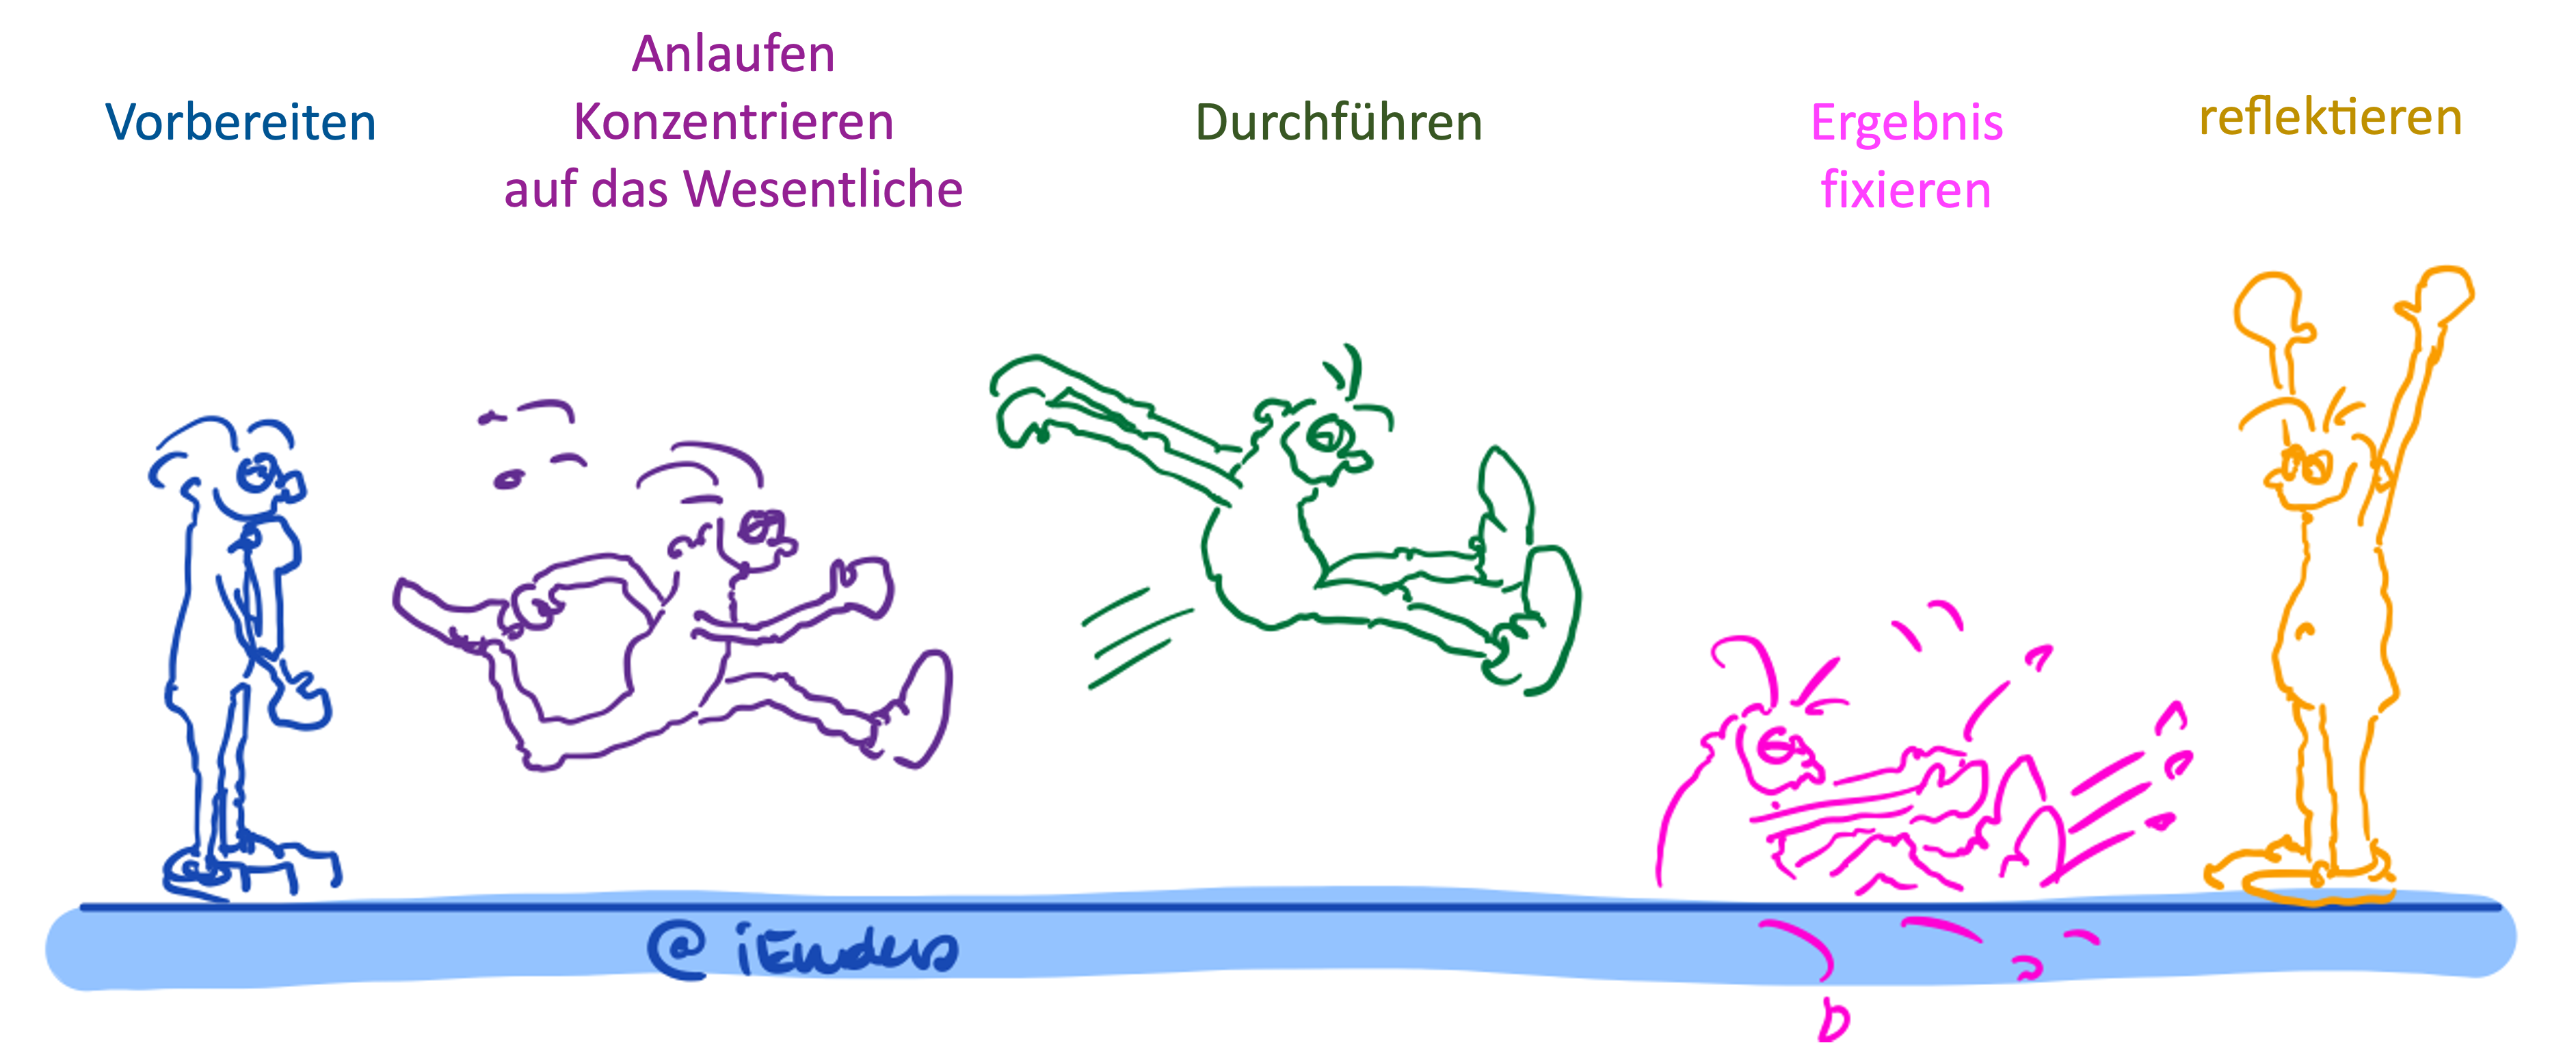
\includegraphics[scale=.5]{Artikulationsschema.png}
	\caption{Grundstruktur eines Artikulationsschemas}
	\label{fig:Artikulationsschema}
\end{figure}


\mip
Insgesamt sind die Schemata als idealtypisch anzusehen und
nicht schablonenhaft zu verwenden
In der Realit\"{a}t treten vielf\"{a}ltige Modifikationen auf:
\begin{itemize}
	\item
	Unterschiedliche Gewichtung der Stufen.
	\item
	Flie{\ss}ender \"{U}bergang oder Verschmelzung von Stufen.
	\item
	Weglassen oder Mehrmaliges Durchlaufen von Stufen.
\end{itemize}

%Vergleichende \"{U}bersicht:
% Siehe \cite[S.\ 200]{BleichrothDahnckeJung}
% \cite[S.\ 215]{Willer}.

Die Struktur von Artikulationsschemata ist grundlegend immer \"{a}hnlich und anschaulich in Abbildung \ref{fig:Artikulationsschema} dargestellt.

\mip
Die in den folgenden Beispielen verschiedenen Schemata \"{a}hneln
einander alle. Es ist eine allgemeine Dramaturgie
wie beim Weitsprung (Vorbereiten -- Anlaufen -- Konzentrieren
auf das Wesentliche -- Durchf\"{u}hren -- Ergebnis fixieren --
reflektieren) oder bei einer
Schulaufsatz-Erlebniserz\"{a}hlung (Einleitung -- Hauptteil -- Schluss) zu erkennen.

\subsection{Herbart: Die Formalstufen}
Die Idee, Unterricht oder allgemeiner: das Lernen, auf diese
Weise planerisch zu gestalten, geht auf Johann Friedrich
Herbart (1776 -- 1841, 1806: Allgemeine P\"{a}dagogik) zur\"{u}ck.
So wird die p\"{a}dagogische Schule, die diese Gedanken (zum Teil
\"{u}berzeichnet-formalisiert) vertritt,
auch die {\em Schule der Herbartianer} genannt.
Ihre wichtigsten Vertreter sind Rhein und Ziller.

\begin{quote}
	\bf Idee: Das Atmen des Geistes
\end{quote}

\begin{enumerate}
	\item
	{\bf Vertiefung (Einatmen)}
	\begin{enumerate}
		\item[1.]
		{\bf Klarheit} Der einzelne Gegenstand wird klar und in allen
		Einzelheiten vor Augen gef\"{u}hrt.
		\item[2.]
		{\bf Assoziation} In freier Gedankenbildung werden alle nur
		denkbaren geistigen Erkenntnisse aus der Erinnerung in
		Verbindung zu den bereits vorhandenen Elementen gesetzt.
	\end{enumerate}

	\item {\bf Besinnung (Ausatmen)}
	\begin{enumerate}
		\item [3.]
		{\bf System} Die Verbindung des erkannten einzelnen zu den
		bisherigen Erkenntnissen wird systematisch aufbereitet, eine
		Einordnung findet statt.
		\item[4.]
		{\bf Methode} Die Erkenntnis wird angewandt, wobei sie sich
		verifiziert.
	\end{enumerate}
\end{enumerate}


\subsection{Heinrich Roth (1963): Die Lernstufen}
Die diesem Lernstufenschema zugrundeliegende Idee besteht
darin, den Lernvorgang des Sch\"{u}lers psychologisch geeignet zu
begleiten. Es gr\"{u}ndet sich letztlich auf umfassende empirische
Studien zu Lernvorg\"{a}ngen.

\mip
Es ist typisch f\"{u}r eine Unterrichtsstunde,
in der eine Erkenntnis oder Einsicht gewonnen werden soll, es
eignet sich insbesondere also f\"{u}r den naturwissenschaftlichen
Unterricht und die Physik.
Andererseits ist das Schema sehr allgemein gehalten, so dass es
vielf\"{a}ltig anwendbar ist.

\begin{enumerate}
	\item {\bf Stufe der Motivation} Zum Begriff der Motivation
	vergleiche weiter unten.
	
	\item {\bf Stufe der Schwierigkeiten}
	\begin{itemize}
		\item Unter Umst\"{a}nden verschr\"{a}nkt mit der Stufe der Motivation.
		\item Es handelt sich um eine Art Innehalten in Form eines
		Zwischenstopps nach der Stufe der Motivation.
		Das Ziel tritt klar vor Augen.
		\item Der Sch\"{u}ler soll sich am Ende des Einstiegs der
		Schwierigkeiten, des Problems, bewusst sein.
		Das zu l\"{o}sende Problem muss isoliert und klar formuliert werden.
		Erste L\"{o}sungsversuche sollten zur\"{u}ckgestellt werden.
		\item Das Problem erscheint
		(evtl. als Thema der Unterrichtsstunde)
		an der Tafel oder auf der Folie.
		\autocite[S. 207]{BleichrothDahnckeJung}
	\end{itemize}
	
	\item {\bf Stufe der L\"{o}sung}
	
	Sie bildet den eigentlichen inhaltlichen Mittelpunkt der Stunde.
	Im Physikunterricht wird hier im allgemeinen experimentiert.
	
	Je nach Unterricht kann die konkrete Ausgestaltung
	unterschiedlich angelegt sein:
	
	\begin{itemize}
		\item Induktive Erarbeitung eines Gesetzes im Experiment
		(Hooke'sches Gesetz, ohmsches Gesetz, Gesetz \"{u}ber die Siedetemperaturerniedrigung bei Druckerh\"{o}hung)
		$\to$ Elementarisierung.
		\item Einsicht in einen technischen Funktionszusammenhang
		(Otto-Motor, Elektromotor, hydraulische Hebeb\"{u}hne, Glasfaserkabel).
		\item Einf\"{u}hrung von Begriffen (Verdunstung, W\"{a}rmeleitung) oder
		Gr\"{o}{\ss}en (Kraft, Spannung), Einheiten und Messverfahren.
		\item Messung einer Konstanten.
	\end{itemize}
	
	\item {\bf Stufe des Tuns und Ausf\"{u}hrens}
	\begin{itemize}
		\item Die Halbleiterdiode, der Elektromotor wird tats\"{a}chlich eingesetzt.
		\item Best\"{a}tigungsversuch.
	\end{itemize}
	
	\item {\bf Stufe des Behaltens und Ein\"{u}bens}
	
	Psychologische Erkenntnis:
	Durch Wiederholung kann das Behalten im
	Ged\"{a}chtnis wesentlich gef\"{o}rdert werden.
	
	\begin{itemize}
		\item (M\"{u}ndliche) Wiederholung (in eigenen Worten)
		\item \"{U}bung, \"{U}bungsaufgaben
		($\to$ Typisch im Mathematikunterricht).
		\item Anwendung in Natur, Alltag und Technik (Verdunstung $\to$
		Schwei{\ss}bildung, Hydraulische Presse $\to$ Autohebeb\"{u}hne,
		3.\ Bewegungsgleichung $\to$ Fahrschulformel)
		\item Variation
		\item Beispiele zu dem Gesetz,
		Spezialf\"{a}lle (Auftrieb $\to$ Schweben).
		\item Eintrag ins (Merk-)Heft.
		\item Hausaufgabe.
		\item Schulbuch-Abgleich.
	\end{itemize}
	
	Beispiel: KnoffHoffShow:
	Nach jeweils einem Thema werden die Inhalte in
	Kurzsequenzen wiederholt.
	
	\item {\bf Stufe der Integration, der \"{U}bertragung und
	der Bereitstellung}
	
	\begin{itemize}
		\item Eventuell Nahtstelle mit Anfangsphase der Folgestunde
		\item Integration (Wagenschein: Herstellung des Systems):
		Der neu gelernte Inhalt wird in das System der fr\"{u}her
		gelernten Inhalte auf vielf\"{a}ltige Weise
		eingef\"{u}gt (Verkn\"{u}pfung, Assoziation, Ordnung,\dots).
		\item \"{U}bertragung des Inhalts auf neue Sachverhalt
		(Beachte: Nach W.\ Jung ist Transfer i.a.\ nur sehr
		beschr\"{a}nkt m\"{o}glich).
		\item Element der Lernzielkontrolle.
	\end{itemize}
\end{enumerate}
	
\subsection{Grob-Phasen gem\"{a}{\ss} \textcite{DuitHausslerKircher}}
\begin{enumerate}
	\item {\bf Motivation} oder Einstiege
	\item {\bf Erarbeitung} Probleml\"{o}sung (beispielsweise im Experiment)
	\begin{enumerate}
	\item
	Planung des Experiments
	\item
	Durchf\"{u}hrung des Experiments
	\item
	Auswertung des Experiments
	\item
	R\"{u}ckblickende Er\"{o}rterung des Experiments
	\item
	Allgemeine Er\"{o}rterung
	\end{enumerate}
	\item {\bf Vertiefung} Integration, Behalten, Transfer.
\end{enumerate}
	
\subsection{H.F.\ Bauer: Experimentalunterricht}
Das Grundschema des entdeckenden Unterrichts wird
hier spezialisiert-differenziert im Hinblick auf
das Experimentieren umgesetzt.

\mip Ziel des Unterrichts ist nicht Forschung an sich, sondern eine
Vertrautheit mit dem Forschen an sich.
	\begin{enumerate}
	\item {\bf Motivation}
	\item {\bf Problemherstellung}
	\item {\bf Meinungsbildung}
	\item {\bf Planen} und Konstruieren
	\item {\bf Laborieren --- Experimentieren}
	\item {\bf Schlie{\ss}en}
	\item {\bf Abstrahieren}
	\item {\bf Wissenssicherung durch Anwendung und \"{U}bung}
\end{enumerate}

\subsection{Kerschensteiner (1914)}
Inspiriert durch John Dewey (1910).
Die zugrundeliegende Idee besteht darin, das Grundmuster
naturwissenschaftlicher Erkenntnis
in Unterrichtsabl\"{a}ufe einzupassen.
\begin{enumerate}
	\item {\bf Problem} Beobachtung, Fragestellung
	\item {\bf Hypothese} Vermutung
	\item {\bf Experiment} Untersuchung
	\item {\bf Verifikation oder Falsifikation} Best\"{a}tigung oder
	Nichtbest\"{a}tigung.
\end{enumerate}

\subsection{\textcite{Ploeger}: Forschender Physikunterricht}

Konkret, anwendungsnah und auf den Punkt gebracht wird dieses Konzept in
\textcite{Ploeger} beschrieben.
Es finden sich dort auch viele Beispiele.
\begin{enumerate}
	\item {\bf Problemfrage}
	\item {\bf Vermutung}
	\item {\bf Versuchsplanung}
	\item {\bf Experiment}
	\item {\bf Auswertung}
\end{enumerate}

% -------------------------------------------------- eingefuegt von A. Enders 8.1.2024 -----------------------------------------------------------------------------------------------------
\subsection{Probleml\"{o}sendes Verfahren -- Das Normalverfahren nach Mothes}

Hans Mothes w\"{a}hlte 1957 f\"{u}r dieses Unterrichtsverfahren die Bezeichnung \glqq Normalverfahren\grqq, da er davon ausging, dass sich die Stufen des Normalverfahrens an die induktive Vorgehensweise der fachwissenschaftlichen Erkenntnisgewinnung anlehnen, n\"{a}mlich Problem, Hypothese, Experiment und Verifikation. Ob jedoch dieses Verfahren tats\"{a}chlich ein Abbild der Wissenschaft ist, ist fraglich, da f\"{u}r Forschung eine Idee notwendig ist, was man \"{u}berhaupt untersuchen will. Im Gegensatz dazu inszeniert der Lehrer den Unterricht h\"{a}ufig so, als w\"{a}ren ihm die zu ermittelnden Sachverhalte noch nicht bekannt. Konkret besteht das Normalverfahren nach Mothes aus folgenden Stufen:

\begin{enumerate}
	\item {\bf Problemfrage}
	\item {\bf Meinungsbildung}
	\item {\bf Die Nachpr\"{u}fung des auf der Stufe der Meinungsbildung gewonnenen Urteils}, welches die Schritte \emph{deduktive \"{U}berlegungen}, \emph{Versuchsplanung},  \emph{eigentliches Experiment} und \emph{Urteil Erkenntnissatz} beinhaltet
	\item {\bf R\"{u}ckkehr vom Gedankenger\"{u}st der Erkenntnis zur Wirklichkeit}
	\item {\bf Ma\ss nahmen zur Festigung des Unterrichtsergebnisses}
\end{enumerate}

% -------------------------------------------------- Ende Einfuegung von A. Enders 8.1.2024 -----------------------------------------------------------------------------------------------------



\subsection{Die Phase der Motivation}
,,motivare'' hei{\ss}t ,,In Bewegung versetzen''.
In der Psychologie ist der Motivationsbegriff nicht einheitlich
definiert.
\bip
Berlyne (1974) sieht den kognitiven Konflikt als Kern der
(sachbezogenen) Motivation an.
Kognitive Konflikte entstehen, wenn sich Wahrnehmungen
nicht in den vorhandenen Wissens- oder Erfahrungszusammenhang
einbetten lassen, sie folgen dabei einigen Grundmustern:

\begin{itemize}
	\item {\bf \"{U}berraschung}
	Konflikt zwischen Erwartung und Erfahrung.
	
	Man erwartet aufgrund gefestigter Erfahrung ein anderes
	Ergebnis als es tats\"{a}chlich erfolgt.
	
	Das Auftreten h\"{a}ngt von der vorhandenen Erfahrung
	(Lebensalter, Jahrgangsstufe) ab.
	\begin{itemize}
		\item
		Ein Schiff aus Eisen geht nicht
		unter (Schwerkraft $\ctr$ Auftrieb).
		\item
		Ein Glas Wasser flie{\ss}t nicht aus, wenn es mit einer St\"{u}ck
		Karton abgedeckt und vorsichtig umgedreht wird
		(Schwerkraft $\ctr$ Adh\"{a}sionskr\"{a}fte).
		\item
		Ein Phasenpr\"{u}fer leuchtet auf, wenn man mit der anderen Hand
		die Wasserleitung ber\"{u}hrt. (Wasserleitung $\ctr$ Erdung)
		\item
		Huckepackball: Ein kleiner Superball wird auf eine gro{\ss}en gelegt,
		beide werden in dieser Lage fallen gelassen.
		Der kleine Ball erreicht nach dem Aufprall ein
		Vielfaches der Ausgangsh\"{o}he
		(Energiesatz $\ctr$ Energie\"{u}bertragung).
		\item
		Wasser in einem d\"{u}nnen R\"{o}hrchen steht h\"{o}her als in der Umgebung.
		(Hydrostatisches Grundgesetz $\ctr$ Kapillarit\"{a}t)
		\item
		Ein Aluminiumring wird vom Pol eines Elektromagneten beim
		Einschalten abgesto{\ss}en
		(Aluminium ist nicht ferromagnetisch $\ctr$ Lorentzkr\"{a}fte).
	\end{itemize}
	
	\item {\bf Zweifel} Konflikt zwischen Glauben und Nichtglauben
	
	Zweifel ensteht bez\"{u}glich einer nicht direkt nachpr\"{u}fbaren
	Aussage, weil sie Resultat einer Idealisierung oder theoretischen
	\"{U}berlegung ist.
	
	\begin{itemize}
		\item
		Ein reibungsfrei beweglicher Wagen f\"{a}hrt gleichf\"{o}rmig weiter,
		wenn er sich selbst \"{u}berlassen wird.
		\item
		Alle K\"{o}rper (auch Menschen) ziehen einander an.
		\item
		Ein G\"{u}terwagen kann mit der Hand gezogen werden.
		\item
		Wir bewegen uns mit \SI{100}{\kilo\meter\per\hour} um die Erdachse und mit \SI{30}{\meter\per\second}
		um die Sonne.
	\end{itemize}
	
	\item {\bf Ungewissheit, Verwirrung}
	Konflikt zwischen mehrdeutigen oder unvollst\"{a}ndigen Erfahrungen.
	
	\begin{itemize}
		\item
		Materie kann als Kontinuum oder als k\"{o}rnige Struktur aufgefasst
		werden.
		\item
		Zieht man am offenen Ende eines Zwirns an einer N\"{a}hfadenrolle,
		so stellt sich die Frage, ob sich die Rolle sich her- oder wegbewegt.
		\item
		Auf einen wasserbedeckten Teller wird eine Kerze gestellt und dann
		ein Glasgef\"{a}{\ss} \"{u}bergest\"{u}lpt.
		Warum steigt das Wasser auf? (Chemische Effekte $\ctr$
		W\"{a}rmeausdehnungseffekte)
		\item
		Historisch: Licht hat Wellen- oder Teilchencharakter.
	\end{itemize}
	
	\item {\bf Irrelevanz}
	Bisherige Informationen sind irrelevant
	Beispiel: Rutherford Streuversuche.
	
	\item {\bf Verunsicherung, Ratlosigkeit}
	\begin{itemize}
		\item
		Kann man zu einem Regenbogen spazieren?
		\item
		Ist ein Lichtstrahl sichtbar?
		\item
		Schwimmt Aluminium im Wasser?
	\end{itemize}
	
	\item {\bf Staunen, Wundern}
	\item {\bf Paradoxie, Zwiespalt}
	
	\begin{itemize}
		\item
		Das Hydrostatische Paradoxon: Bei gleicher Wasserh\"{o}he ist der
		Druck am Boden eines Gef\"{a}{\ss}es unabh\"{a}ngig von Volumen oder Form
		des Gef\"{a}{\ss}es.
		\item
		Das Aerodynamische Paradoxon: Man bl\"{a}st durch den Spalt zwischen
		zwei einander zugewandt gew\"{o}lbten Kartons.
		Die Kartons bewegen sich aufeinander zu.
		(Statischer Druck $\ctr$ Staudruck).
		
		\item
		Das Zwillingsparadoxon der Allgemeinen Relativit\"{a}tstheorie.
		
		\item
		Historisch: Olbers'sches Paradoxon (1826).
	\end{itemize}
	
	\item {\bf Neuigkeitsgehalt, Aktualit\"{a}t}
\end{itemize}

\subsection{Einstiege in eine Unterrichtseinheit}

Dieser Begriff ist weniger anspruchsvoll als der der Motivation.
Mit dem Einstieg nimmt der Unterrichtsgang den Anfang eines
roten Fadens (des Lernprozesses) auf.

Spielarten von Einstiegen:
\begin{itemize}
	\item
	Einstieg \"{u}ber eine Beobachtung in der Natur.
	\begin{itemize}
		\item
		Lichtstrahlen im Wald.
		\item
		Regenbogen.
	\end{itemize}

	\item
	Einstieg \"{u}ber eine Beobachtung im Haushalt
	\begin{itemize}
		\item
		Dampfkochtopf, K\"{u}hlschrank, Fernseher, Heizung.
		\end{itemize}
		
		\item
		Einstieg \"{u}ber eine Beobachtung in der Freizeit.
		\begin{itemize}
		\item
		Fahrrad, Schwimmen.
	\end{itemize}
	
	\item
	Einstieg \"{u}ber Handwerk und Technik.
	\begin{itemize}
	\item
	Metallbau: Schwei{\ss}en, Korrosion.
	\item
	Elektro: Installation
	\item
	Bau: Kran, Hydraulische Maschinen, W\"{a}rmeisolation, \dots
	\end{itemize}
	
	\item
	Einstieg \"{u}ber eine (qualitative oder quantitative)
	Versuchsreihe.
	\begin{itemize}
	\item
	Welche Stoffe leiten den el.\ Strom?
	\item
	Hooke'sches Gesetz.
	\item
	Ohm'sches Gesetz.
	\end{itemize}
	
	\item
	Einstieg \"{u}ber einen Schl\"{u}sselbegriff oder -gegenstand.
	
	\item
	Einstieg \"{u}ber ein aktuelles Ereignis
	\begin{itemize}
	\item
	Baugenehmigung f\"{u}r Physik-Projekt (Garching),
	\item
	Bau eines Kraftwerks, \"{U}berlandleitung,
	\item
	Weltraumfahrt (Marslandung)
	\item
	Astronomie (Finsternisse, Kometen,\dots)
	\end{itemize}
	
	\item
	Einstieg \"{u}ber Vergegenw\"{a}rtigung einer historischen Begebenheit
	(z.B.\ wegen Jahrestag einer Entdeckung, Briefmarkenherausgabe,
	Biographie eines Naturforschers)
	\begin{itemize}
	\item
	Oersted-Versuch: Induktion in ruhenden Leitern.
	\item
	Newton'sches Gravitationsgesetz.
	\item
	Entdeckung der Radioaktivit\"{a}t: Bequerel.
	\item
	Erfindung des ersten Transistors: 23.12.1947.
	\item
	Auffindung der R\"{o}ntgenstrahlung: 7.11.1895.
	\end{itemize}
	
	\item
	Einstieg \"{u}ber ein Ereignis im Jahreslauf
	(Bleigie{\ss}en an Silvester, Feuerwerk, Asphaltspiegelungen im Sommer)
	
	\item
	Einstieg \"{u}ber ein pers\"{o}nliches Erlebnis.
	
	\item
	Einstieg \"{u}ber einen Zeitungs- oder Zeitschriftenartikel, Radio- oder Fernsehbericht, Buchlekt\"{u}re.

\end{itemize}

\subsection{Das Aufstellen einer Vermutung bzw. Hypothese}
Im Sinne Kerschensteiners  steht vor der schnellen Beantwortung einer
Frage an die Natur durch das Experiment die Aufstellung m\"{o}glicher Ergebnisse
\bip
Beispiele:
\begin{itemize}
\item
Fadenpendel: Welche Gr\"{o}{\ss}en sind entscheidend?
\item Parallelschaltung. Welcher Gesamtwiderstand ergibt sich,
wenn zwei Widerst\"{a}nde parallel geschalten werden? Vermutungen:
    \begin{itemize}
      \item Mittelwert $\frac{R_1 + R_2}2$,
      \item $\frac{R_1+R_2}4$,
      \item $R_1 \cdot R_2$,
      \item $\frac{1}{R} = \frac{1}{R_1} + \frac{1}{R_2}$.
    \end{itemize}
\item Widerstand eines Drahtes. Von welchen Gr\"{o}{\ss}en h\"{a}ngt er ab?
\item Mondphasen:
\begin{itemize}
  \item Erdschatten,
  \item Halbseitiges Leuchten,
  \item Halbseitige Beleuchtung durch die Sonne.
\end{itemize}
\item \"{A}therhypothese,
\item Kontinuumshypothese.
\item Museum f\"{u}r Mensch und Natur in M\"{u}nchen: Der Besucher (Kind) muss erst
seine Vermutungen \"{u}ber bestimmte Fragen:
\begin{itemize}
\item Welche der gezeigten Tiere sind Fr\"{o}sche?
\item Welche der gezeigten Tiere haben Knochen?
\item Welche Tiere sind am schnellsten?
\end{itemize}
\"{a}u{\ss}ern, bevor die Frage aufgel\"{o}st wird.
\end{itemize}


%------------------------------------------------------------------------------------------------------------------------------------------------------------------------
\bip\bip
\section{Unterrichtsverfahren}\label{Verfahren}

Synonym werden auch die Begriffe
,,Methodenkonzept'', ,,Methodisches Konzept'' oder ,,Unterrichtsgang'' verwendet.
Unterrichtsverfahren beschreiben nicht so sehr den zeitlichen Ablauf,
sondern eher den grundlegenden Ductus (Gang) eines Unterrichts.
Empirische Untersuchungen zum Erfolg der Unterrichtsverfahren
sind schwierig, sie erfolgen an simplifizierten Verfahren.

\mip
Es besteht ein grundlegendes Spannungsfeld:
\mip
\begin{center}
\begin{tabular}{ |p{7cm}| p{7cm}| }
\hline
 Entdeckender Unterricht
&
Darbietender Unterricht
\\ \hline \hline
 Probleml\"{o}sendes Unterrichtsverfahren
&
Darstellend-entwickelndes Unterrichtsverfahren
\\ \hline
 Die Sch\"{u}ler bet\"{a}tigen sich selbst als ,,Physik-Erkennende''.
&
Die Sch\"{u}ler lernen (rezipieren) den Lernstoff.
\\ \hline
 Prozessziele (Methodische Denken) &
Konzeptziele (Wissen, Kenntnisse)
\\ \hline
 Idealform, aufw\"{a}ndig
&
Realit\"{a}tsbedingt, \"{o}konomisch
\\ \hline
 Weniger Lenkung, intrinsische Motivation
&
Mehr Lenkung
\\ \hline
 Eher Sch\"{u}lerversuche
&
Eher Lehrerversuche
\\ \hline
 Exponent: J.\ Bruner (am): Gedanken zu einer Theorie des Unterrichts
,,Entdeckenden Lernens''. &
Exponent: D.J.\ Ausubel (kan): Psychologie des Unterrichts
\\ \hline
 Medieneinsatz: Experimente, Materialien aus dem Alltag
&
Medieneinsatz: Vorausorganisatoren, Arbeitsbl\"{a}tter
\\ \hline

{Besondere Auspr\"{a}gungen: \newline
Genetischer Unterricht \newline
Forschender Unterricht \newline
Nacherfindender Unterricht \newline
Historisierender Unterricht \newline
Modellmethode
}
&
{Besondere Auspr\"{a}gungen: \newline
Sinnvoll-\"{u}bernehmender Unterricht \newline
Fragend-entwickelnder Unterricht \newline
Nachmachender Unterricht \newline
Induktiv-deduktives Verfahren \newline
Synthetisch-analytisches Verfahren
}
\\ \hline
\end{tabular}\end{center}

Langfristig wird ein Physikunterricht von einer
Verschr\"{a}nkung und Variation dieser beiden grundlegenden
Formen gepr\"{a}gt sein.

\bip\bip
\section{Das genetische Unterrichtsverfahren}

Begr\"{u}nder und spirtus rector: Martin Wagenschein.
\bip
\begin{tabular}{r p{12cm}}
1896 &  Geburt. Studium der Physik und Mathematik,
Promotion in Physik.
\\
$\approx$1920 &  Unterricht an staatlichen Gymnasien,
Erfahrungen in der ,,Freien Schulgemeinde Odenwaldschule''
Paul Geheebs.
\\
1945 &  Schulversuche, Bildungspl\"{a}ne.
\\
1951 &  T\"{u}binger Resolution.
\\
1960--65 &  Ausschuss ,,H\"{o}herer Schule'' des Deutschen Ausschusses.
\\
1956 -- &  Honorarprofessor T\"{u}bingen, 20 Jahre Seminar.
\\
1978 &  Ehrendoktor TH Darmstadt.
\\
Ostern 1988 &  gestorben.
\end{tabular}

\bip
Drei Aspekte des genetischen Unterrichts:
\begin{itemize}
\item Individual-genetischer Aspekt: Die Genese der Erkenntnis im
Sch\"{u}ler.
\item Logisch-genetischer Aspekt: Die allgemeine Genese der
Erkenntnis.
\item Historisch-genetischer Aspekt: Genese der Erkenntnis in der
Entwicklung der Wissenschaft.
\end{itemize}

\bip
Thesenartige Umschreibung der ,,Botschaft'' Wagenscheins:
\begin{itemize}

\item Physikalisches Handeln entfaltet p\"{a}dagogische  Wirkung
schlechthin. Physik ist nicht einfach ein Transportgut der P\"{a}dagogik.

\item Physik braucht Freiraum (von Schulsystem, Lehrpl\"{a}nen,
Zeitzw\"{a}ngen, Vollst\"{a}ndigkeitsbestreben.
\item Der Physikunterricht muss sich auf die Trias
\begin{quote}
Exemplarisch --- sokratisch --- genetisch
\end{quote}
gr\"{u}nden.


\item Exemplarisch: Der Prozess des Werdens von Physik im Menschen
wird anhand von Beispielen erlebt.
Ein einzelnes Ergebnis (Erkenntnismethode,
Arbeitsform) ist repr\"{a}sentativ f\"{u}r das System der Gesamtphysik.
\item Sokratisch  (Sokrates-Dialoge, von Platon \"{u}berliefert):
Der Lernende findet die L\"{o}sung selbst, begleitet durch geschickte
Fragen und Impulse, keine Mitteilung von Informationen.


\item Genetisch:

Physik ist ein Prozess, nicht eine Wissenssammlung:
\begin{quote}
Verstehen (lernen) statt Wissen (lernen)  (Genetisch statt
Enzyklop\"{a}disch)
\end{quote}
(Pestalozzi: Die Schule bringt dem Menschen das Urteil in den Kopf,
ehe er die Sache sieht und kennt.)
\mip
Genetischer Unterricht ber\"{u}cksichtigt das, was die
Sch\"{u}ler schon wissen, er verfr\"{u}ht keine Ergebnisse, sondern zielt
auf deren Einwurzelung, ohne die es keine Formatio gibt.
(Zitat: \cite[S.\ 107 oben]{DuitHausslerKircher}).

\item ,,Rettet die Ph\"{a}nomene'' Die Sch\"{u}ler m\"{u}ssen die Welt
erleben, bevor sie sie (analytisch) erkl\"{a}rend durchdringen
\autocite[S.\ 90,104]{WagenscheinNSV}.

\item Die Selbstzweck-Mathematisierung muss zur\"{u}ckgefahren werden.

\item Die drei Phasen des e-g-s Unterrichts:
\begin{enumerate}
\item Einstieg: \say{Wir steigen vom Seltsamen ins Elementare (von
der Todesschleife zum Tr\"{a}gheitssatz) hinab.}
\autocite[S.\ 205]{WagenscheinPDP}
\item Bildung und \"{U}berpr\"{u}fung von Hypothesen,
\item Vertiefung, Systematisierung (wenig betont in Wagenscheins
Beispielen)
\end{enumerate}

\item Organisatorisch: Mindestens Doppelstunden, besser
Epochalunterricht, Sch\"{u}ler gruppieren sich seminarartig um die
Tische.
\end{itemize}

\bip\bip
\section{Forschender Unterricht}
\subsection{Georg Kerschensteiner}

\begin{tabular}{r p{12cm}}
29.7.1854 &
Geboren in M\"{u}nchen, Ausbildung zum Volksschullehrer,
sp\"{a}ter Gymnasiallehrer.
\\
1874 -- 1880 &  Lehrer an Volksschulen und Gymnasien
in/bei M\"{u}nchen, Augsburg, N\"{u}rnberg, Schweinfurt, M\"{u}n\-chen.
\\
1884 &  Doktorarbeit in Mathematik
\\
1885 -- 1919 &  Leiter des Volks- und Berufsschulamtes,
Stadtschulrat, \"{U}berdenken der Organisation des Schulwesens.
\\
1910 &  Mitinitiator einer Lehrplanreform, die die Bedeutung des
naturwissenschaftlichen Unterrichts
hervorhebt.
(Ausl\"{o}sung des ,,M\"{u}nchner Schulstreits'').
\\
1914 &  \say{Wesen und Wert des naturwissenschaftlichen
Unterrichts}.
\\
1919 -- 1928 &  Universti\"{a}tsprofessor, theoretische Arbeit,
Reisen in die USA, tr\"{a}gt zur Reform des Schulwesens bei.
\\
1926 &  Hauptwerk ,,Theorie der Bildung''.
\\
15.1.1932 &  Gestorben in M\"{u}nchen.
\end{tabular}

\subsection{Kerngedanken seines p\"{a}dagogischen Programms}
Kerschensteiners Ideen bedeuten insgesamt eine Antwort auf das
im 19.\ Jahrhundert vorherrschende Humboldt'sche Bildungsideal
mit seiner geistig-intellektuellen humanistischen
Ausrichtung, das auch die Schullandschaft pr\"{a}gte.
\begin{itemize}
\item Betonung auch der Handarbeit: K\"{o}rperliche Fertigkeiten sind
ein Bestandteil der Menschenbildung.
$\to$ Werkunterricht, Zeichenuntericht, Arbeitsschulbewegung.
\item Begr\"{u}ndung des naturwissenschaftlichen Unterrichts und
seines Bildungswerts.
Naturwissenschaften sind integraler Bestandteil der Menschenbildung.
\item Betonung der naturwissenschaftlichen Methode der
Erkenntnisgewinnung im Unterricht.
$\to$ Forschender Unterricht, siehe unten.
\item Betonung der Berufsbildung: Zur Berufsausbildung geh\"{o}rt
eine umgebende allgemeinere Geistesbildung.
$\to$ Kerschensteiner ist der ,,Vater der Berufsschule''.
\item Soziale Bildung: Ausbildungsziel in der (Berufs-)Schule ist
der ,,Staatsb\"{u}rger in Verantwortung'' $\to$ Sozialkundeunterricht.
\item Selbstt\"{a}tigkeit  $\to $ Sch\"{u}lerexperimente.
\item Anschauung, au{\ss}erschulische Lernorte!
\item Reform des Schulwesens, Umgestaltung der Forbildungsschulen
in Berufsschulen.
\item Kritik: Vernachl\"{a}ssigung der geschichtlichen und
musischen Bildung.
\end{itemize}

\subsection{Die Idee des forschenden Unterrichts}
Auch: Discovery learning, die historischen Wurzeln:
Kerschensteiner, Dewey, Kilpatrick.
\begin{itemize}
\item Orientiert an Methoden der Erkenntnisgewinnung in der Physik.
\item
Abfolge von: Problem -- Hypothese -- Verifikation/Falsifikation.
(Vgl.\ auch das Stufenschema von H.F.\ Bauer bzw.\ Pl\"{o}ger).
\end{itemize}

\bip\bip
\section{Nacherfindender Unterricht}
\begin{itemize}
\item Die Fragestellung besteht in der Konstruktion eines
technischen Ger\"{a}tes,
\item Beispiele: El.\ Klingel, Elektromagnet, Flaschenzug,
Messger\"{a}t, Thermometer, Morse-Apparat, optische Ger\"{a}te,
hydraulische Presse, Kaffeemaschine.
\item Artikulation:
\begin{enumerate}
\item Es werden Pl\"{a}ne entworfen.
\item \"{U}berdenken der Realisierungsm\"{o}glichkeiten.
\item Tats\"{a}chliche Konstruktion
\item Funktionstest
\item Verbesserung des Ger\"{a}tes: Wie kann es einfacher, stabiler,
billiger, bedienungsfreundlicher, zuverl\"{a}ssiger, energiesparender,
umweltfreundlicher gestaltet werden?
\item Das Prinzip der Handlungsorientierung wird verwirklicht.
\item Lernziele bestehen in dem Bewusstsein, dass technische Ger\"{a}te
leichter durchschaubar sind, als man vermutet (vgl.\ auch
BlackBoxPrinzip).
\item Problem: Sch\"{u}lerbaupl\"{a}ne sind komplex angelegt, sie sind
vergleichsweise schwer umsetzbar.
\end{enumerate}
\end{itemize}

%\section{Fragemethode}
%\begin{itemize}
%\item Es handelt sich um eine stark formalisierte
%,,Was-bin-ich-Strategie''.
%(Erinnerung: Sokratischer Unterricht)
%\item Der Lehrer antwortet nur mit ,,Ja'' oder ,,Nein''.
%\item Das Lernziel besteht in ,,Zielgerichtetem Fragen''.
%\item Interessant ist diese Methode bestenfalls als spielerische
%Abwechslung oder f\"{u}r empirische Studien.
%\end{itemize}

\bip\bip
\section{Historisierender Unterricht}

Der historisierende Unterricht ist eine didaktische Methode, bei der Sch\"{u}ler
die Entwicklung wissenschaftlicher Konzepte und Theorien nachvollziehen, indem sie die historischen Schritte und Denkprozesse, die zu unserem heutigen Wissen gef\"{u}hrt haben, studieren. Dies erm\"{o}glicht ein tieferes Verständnis der Natur wissenschaftlicher Erkenntnis, weil es zeigt, wie sich wissenschaftliche Modelle im Laufe der Zeit durch neue Experimente und Theorien verändert haben.
\mip
\textbf{K\"{o}nigsbeispiel:} Entwicklung der Atommodelle: Demokrit und die Idee der Unteilbarkeit (ca 400 v. Chr.) $\to$ Daltons Atomtheorie (1803) $\to$ Thomsons {\glqq}Rosinenkuchenmodell{\grqq} (1897) $\to$ Rutherfords Atommodell (1911) $\to$ Bohrsches Atommodell (1913) $\to$ modernes Atommodell und die Quantenmechanik (20. Jh.)

\bip\bip
\section{Induktiv-deduktives Verfahren}
Die Physik heute besteht in einer Verbindung von
induktiv-empirischer Erkenntnismethode und
deduktiv-mathematischem Schlie{\ss}en.

\mip
Beispiel: Deduktiv:  Reflexionsgesetz  $\to$ Spiegelbild.
Induktiv: Spiegelbilder $\to$ Reflexionsgesetz.

\subsection{Das induktive Verfahren}

inducere (lat.): herauff\"{u}hren, hineinf\"{u}hren.

\mip
{\bf Naturwissenschaftlicher Aspekt} Galileo Galilei  (1564 - 1642),

,,Vom Speziellen zum Allgemeinen''.
Es werden einzelne eindeutig definierte (separierte) Ph\"{a}nomene
untersucht, die Einzelergebnisse f\"{u}hren schrittweise
mosaikartig zu einer umfassenderen (allgemeing\"{u}ltigen) Aussage.


\bip
{\bf Philosophisch-erkenntnistheoretischer Aspekt}
Francis Bacon (von Verulam, 22.1.1561 -- 9.4.1626),
Philosoph, Politiker (Lordkanzler).

\begin{itemize}
\item Begr\"{u}nder des englischen Empirismus im zweiten Teil seines
Hauptwerks ,,Novum Organon'' (1620), der die Geisteswelt der
mittelalterlichen Scholastik zu \"{u}berwinden sucht.
\item Empirismus: Erkenntnis ist allein durch Erfahrung
(Beobachtung der Wirklichkeit) m\"{o}glich.
\item Induktion: Die G\"{u}ltigkeit allgemeiner Urteile wird
durch Induktion (Erfahrung $\to$ Allgemeines Urteil)
begr\"{u}ndet.
\item Auf der geistes\-ge\-schicht\-lichen Grundlage
des Empirismus gedieh die auch heute noch g\"{u}ltige Methode der
naturwissenschaftlichen Erkenntnis (Newton, Boyle).
\item Philosophische Erben: John Locke, Thomas Hobbes,
sp\"{a}ter Positivismus.
\item
Vertreter in der P\"{a}dagogik und Naturwissenschafts\-didaktik:
Kerschensteiner.
\end{itemize}

In Bezug auf die Physikdidaktik und Unterrichtspraxis ist hier gemeint,
dass von einem oder einigen experimentellen Befunden auf ein
allgemeing\"{u}ltiges physikalisches Gesetz geschlossen wird.
Man spricht auch von dem \textit{induktiven Schluss}.

Die Idee f\"{u}r die Ausgestaltung des Experiments kann sich auf
verschiedene Vorerfahrungen st\"{u}tzen.

\begin{itemize}
\item Intuition,
\item Analogien,
\item Pr\"{a}zisierung einer qualitativen Beobachtung oder eines
fr\"{u}heren Experiments,
\item eine oder mehrere durch Nachdenken gewonnene Hypothesen.
\end{itemize}

\bip Beispiel f\"{u}r einen induktiven Schluss: \\[2ex]
Ein Kupferrohr dehnt sich bei Erw\"{a}rmung aus \\
$\Rightarrow$ \q Alle K\"{o}rper dehnen sich bei Erw\"{a}rmung aus. \\
\mip
Es gibt aber die Anomalie des Wassers, Dichtemaximum bei \SI{4}{\celsius}.
\bip
Der induktive Schluss ist erkenntnistheoretisch eigentlich
nicht zul\"{a}ssig. (Kritik an der induktiven Methode durch Karl Popper).

\subsection{Das deduktive Verfahren}

deducere (lat): herabf\"{u}hren.

\mip
{\bf Naturwissenschaftlich-mathematischer Aspekt},

,,Vom Allgemeinen zum Speziellen.''
Ausgehend von allgemeinen feststehenden Gesetzen (Axiomen)
wird auf Eigenschaften und Gesetzm\"{a}{\ss}igkeiten von einzelnen
Beispielen geschlossen.

\bip
Dieses Prinzip ist vor allem in der Mathematik stark verwirklicht.
Ausgehend von Axiomen (\"{u}ber bestimmte Zahlbereiche zum Beispiel)
werden S\"{a}tze \"{u}ber diese Zahlen abgeleitet (deduziert).
Konkret bedeutet dies das Beweisen in der Mathematik.
\mip
Historisch: Euklid: Seine axiomatische Grundlegung der Geometrie in den
,,Elementen''.
\mip
Heute wird die Mathematik durch Logik und Mengenlehre grundgelegt.
Alle anderen Strukturen werden daraus erschlossen.

Beispiele aus der Physik:
\begin{itemize}
\item Maxwellgleichungen der Elektrodynamik
             $\to$ Wellenoptik $\to$ Geometrische Optik.
\item Grundgesetz der Mechanik $\to$ Tr\"{a}gheitssatz.
\item Der Energieerhaltungssatz als ein grundlegendes Prinzip erm\"{o}glicht
die Beschreibung und Deutung unterschidelichster Ph\"{a}nomene der Physik.
\item GUT (Grand Unified Theory):
Alle vier ,,Urkr\"{a}fte'' werden aus einer
einzigen ,,allgemeinen Theorie der Kraft'' gewonnen.
\end{itemize}

\bip\bip
\section{Sinnvoll \"{u}bernehmender Unterricht}

Die lerntheoretische Begr\"{u}ndung erfolgte durch
David P.\ Ausubel (1974):

Hier ist ein Unterricht auf der Grundlage eines
eher mitteilenden Lehrens und rezeptiven Lernens
gemeint, das von einem rein ,,mechanischen''
Lernen abgegrenzt aufzufassen ist.
Die zu erlernenden Konzepte werden ,,sinnvoll''
zu einem Netz zusammengef\"{u}gt bzw.\ in das Netz des Vorwissens
eingef\"{u}gt.
\bip
Es handelt sich um einen Konzeption, die auch den eher \"{o}konomischen
Erfordernissen der Schulpraxis entgegenkommt.
\bip
Methodisches Kennzeichen des sinnvoll \"{u}bernehmenden Unterrichts
sind die {\it Vorausorganisatoren (advance organizer)}.
Es handelt sich dabei, wie der Name sagt, um die Aufarbeitung
des vorhandenen Wissens und seine Bereitstellung in einem
\"{U}berblick.
\bip
Zitat: These organizers are introduced in advance of
learning itself, and are also presented at a higher level
of abstraction, generality, and inclusiveness; and since
the substantive content of a given organizer or
series of organizers is selected on the basis of its
suitability for explaining, integrating, and interrelating the
material they precede, this strategy simultaneously satisfies the
substantive as well as the programming criteria for enhancing
the organization strength of cognitive structure.
\bip
Die Abfolge in einem sinnvoll \"{u}bernehmender Unterricht
kann wie folgt beschrieben werden:
\begin{itemize}
\item Einstieg: Advance Organizers
\item Erarbeitung: Die Lerninhalte werden dargeboten.
Verwandte Inhalte werden zun\"{a}chst unabh\"{a}ngig dargestellt.
\begin{itemize}
\item Fortschreitende Differenzierung,
\item Festigung,
\item Integrative Auss\"{o}hnung.
\end{itemize}
\item Vertiefung.
\end{itemize}



